\documentclass{beamer}

\usepackage[utf8]{inputenc}
\usepackage{graphicx}
%\usepackage{amsmath}
\graphicspath{ {./images/} }
\usepackage{subcaption}

\usepackage{enumitem}
\setlist{itemsep=10pt}
\setitemize{label=\usebeamerfont*{itemize item}%
  \usebeamercolor[fg]{itemize item}
  \usebeamertemplate{itemize item}}

%Information to be included in the title page:
\title{Abelian Sandpile Basics}
%\author{Anonymous}
%\institute{ShareLaTeX}
\date{2018}



\begin{document}

\frame{\titlepage}

\begin{frame}
\frametitle{Abelian Sandpile Model}
\begin{itemize}
\item Rough model of a pile of sand, based on a finite directed (multi-) graph $G$, with vertices $V$ and edges $E$.

\item Chips (grains of sand) are stacked on the vertices.

\item Chips can flow to other vertices via edges of $G$.

\item Originally studied on uniform grids.

\item Also known as the chip-firing game.
\end{itemize}
\end{frame}

\begin{frame}
\frametitle{Chip-Firing}
\begin{itemize}
\item Let $n_i$ be the number of chips on vertex $v_i$
\item Let $e_{i} = \{e \in E : e \mbox{ starts at } v_i\}$

\item If a vertex $n_i \geq |e_{v_i}|$ it can \textbf{fire}.

\item When a vertex fires, it transfers a chip down each of its \textbf{outbound} edges.
\end{itemize}


\end{frame}

\begin{frame}
\frametitle{Chip-Firing Example}

%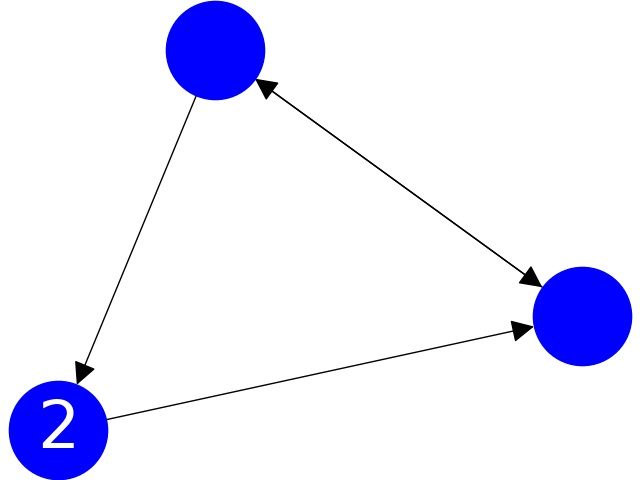
\includegraphics[width=0.5\textwidth]{sandpile_simple_0}%
%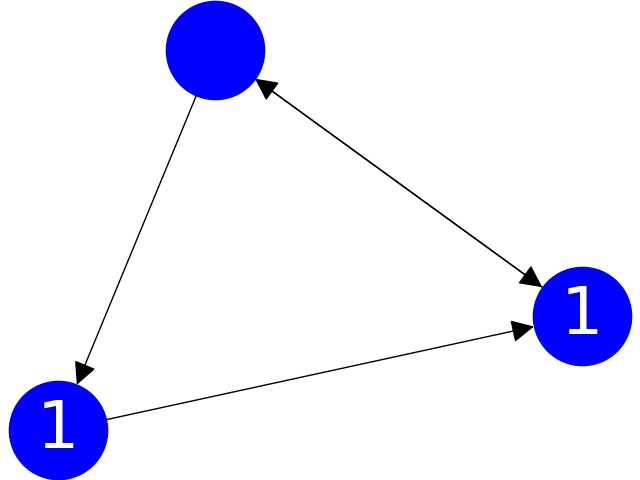
\includegraphics[width=0.5\textwidth]{sandpile_simple_1}

\begin{figure}[h!]
  \centering
  \begin{subfigure}[b]{0.4\linewidth}
    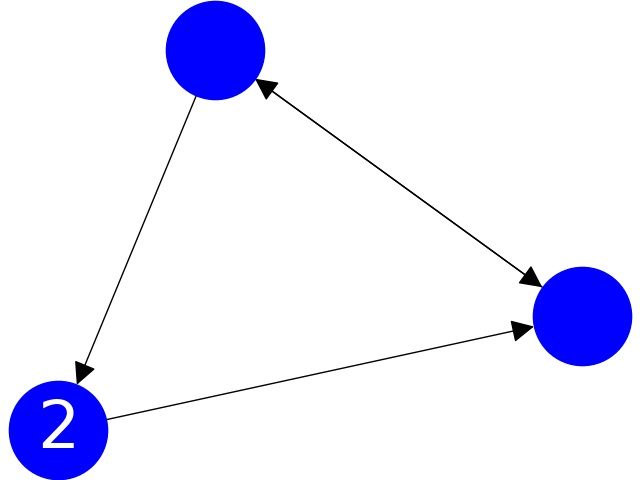
\includegraphics[width=\linewidth]{sandpile_simple_0}
    \caption{Before firing: Lower left vertex has one outbound edge and two chips.}
  \end{subfigure}
  \begin{subfigure}[b]{0.4\linewidth}
    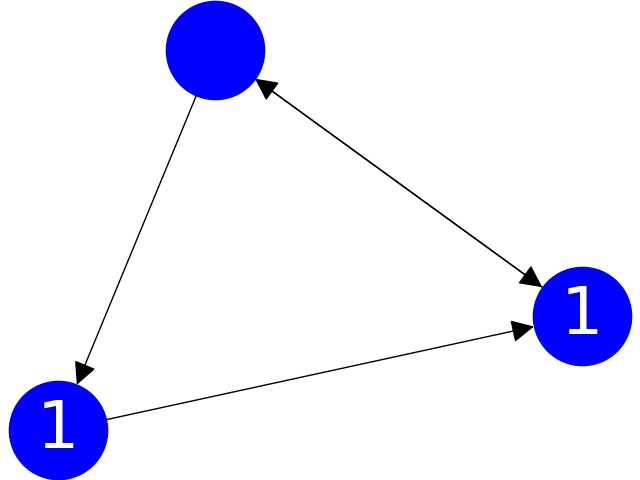
\includegraphics[width=\linewidth]{sandpile_simple_1}
    \caption{After firing: One chip has been transferred to the far right vertex.}
  \end{subfigure}
  \caption{Firing example.}

\end{figure}

\end{frame}


\begin{frame}
\frametitle{Chip Configuration}

\begin{itemize}
\item A \textbf{configuration} is the set of pairs $\{(v_i,n_{i,t}) : v_i \in V\}$, where $n_{i,t}$
is the number of chips on $v_i$ at time/iteration $t$.

\item If we fix an ordering of $V$, use a vector: $c_t = (n_{0,t},n_{1,t},...,n_{N,t})$
\end{itemize}

\begin{figure}[h!]
  \centering
  \begin{subfigure}[b]{0.4\linewidth}
    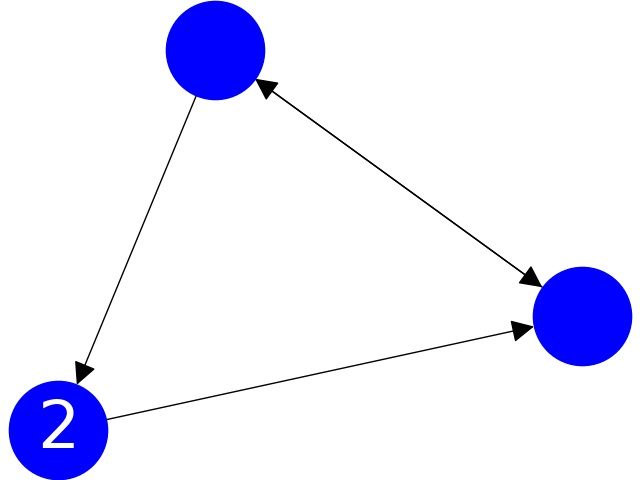
\includegraphics[width=\linewidth]{sandpile_simple_0}
    \caption{$c_0 = (2,0,0)$}
  \end{subfigure}
  \begin{subfigure}[b]{0.4\linewidth}
    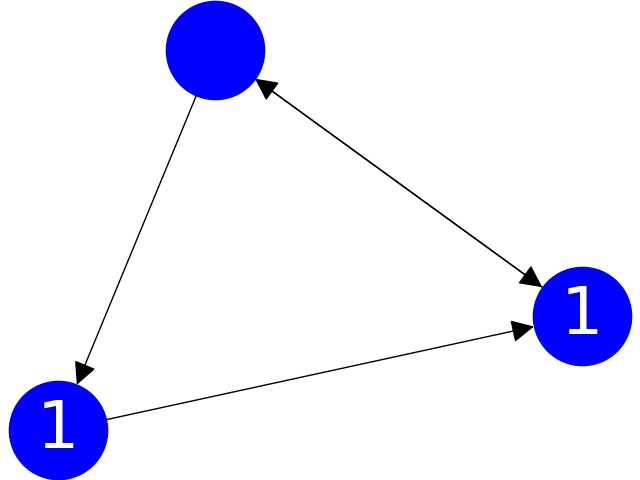
\includegraphics[width=\linewidth]{sandpile_simple_1}
    \caption{$c_1 = (1,1,0)$}
  \end{subfigure}
  \caption{Vertices indexed counter-clockwise starting from lower left vertex}

\end{figure}

\end{frame}

\begin{frame}
\frametitle{Does it Stabilize?}

\begin{itemize}

\item A configuration is \textbf{stable} if none of the vertices can be fired, e.g.
$n_i < |e_{v_i}| $ $ \forall $ $i$.
\item \textbf{Stabilization} is a sequence of vertex firings that result in a stable configuration.
\end{itemize}

\begin{figure}[h!]
  \centering
  \begin{subfigure}[b]{0.4\linewidth}
    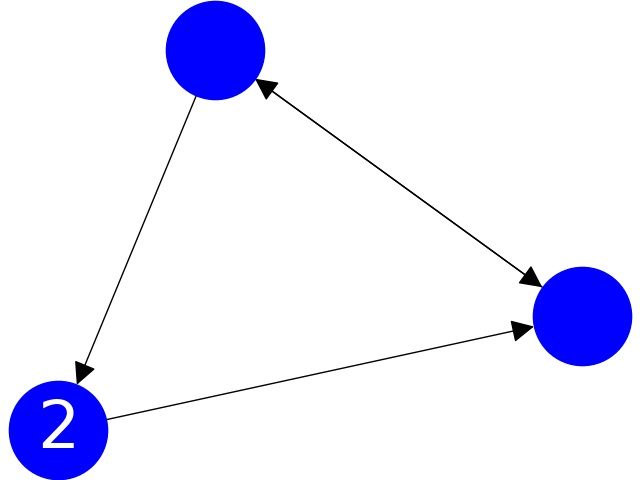
\includegraphics[width=\linewidth]{sandpile_simple_0}
    \caption{$c_0 = (2,0,0)$}
  \end{subfigure}
  \begin{subfigure}[b]{0.4\linewidth}
    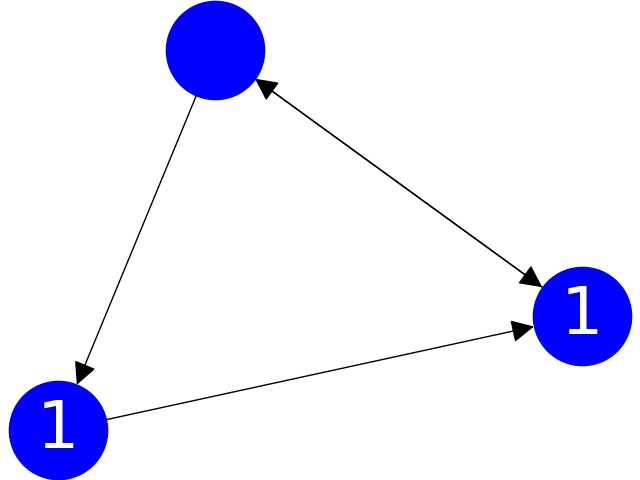
\includegraphics[width=\linewidth]{sandpile_simple_1}
    \caption{$c_1 = (1,1,0)$}
  \end{subfigure}

\end{figure}


\end{frame}


\begin{frame}
\frametitle{Is it stable?}


\begin{figure}[h!]
  \centering
  \begin{subfigure}[b]{0.4\linewidth}
    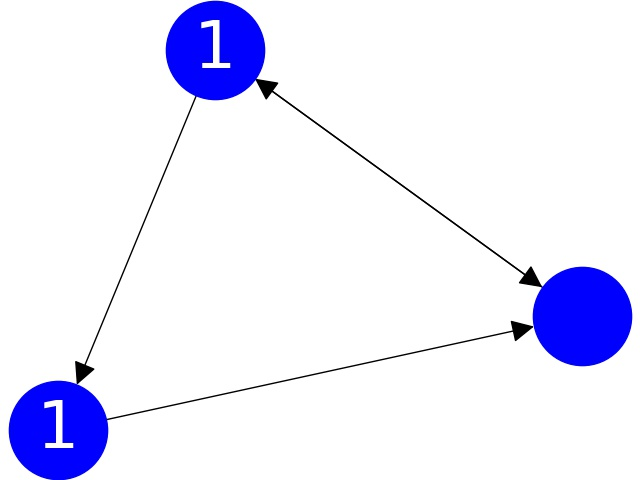
\includegraphics[width=\linewidth]{sandpile_simple_2}
    \caption{$c_2 = (1,0,1)$}
  \end{subfigure}
  \begin{subfigure}[b]{0.4\linewidth}
    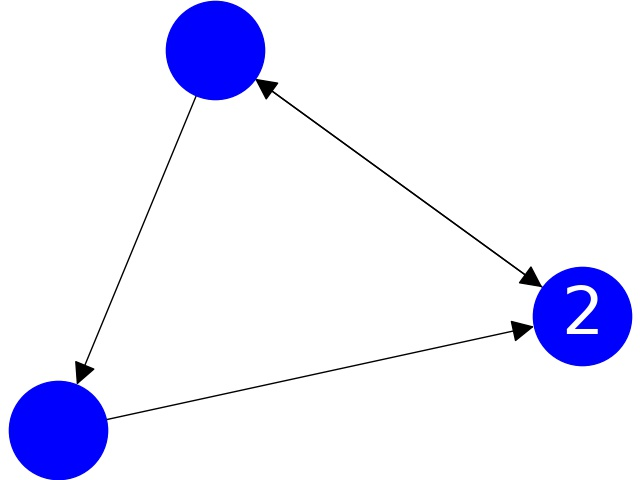
\includegraphics[width=\linewidth]{sandpile_simple_2p}
    \caption{$c_{2'} = (0,2,0)$}
  \end{subfigure}
\end{figure}

\begin{figure}[h!]
  \centering
  \begin{subfigure}[b]{0.3\linewidth}
    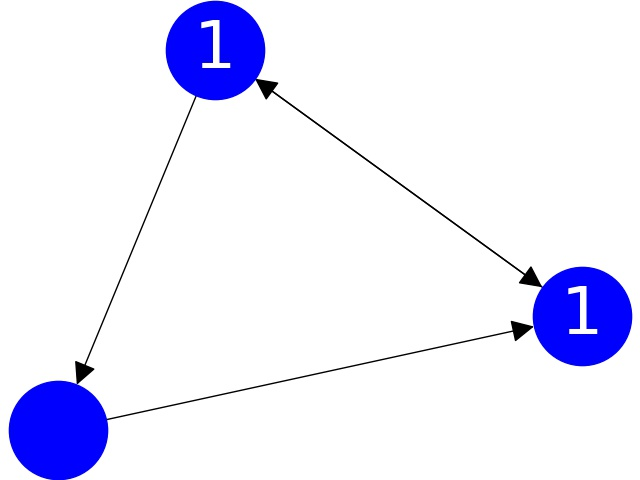
\includegraphics[width=\linewidth]{sandpile_simple_3}
    \caption{$c_{3} = (0,1,1)$}
  \end{subfigure}
  \begin{subfigure}[b]{0.3\linewidth}
    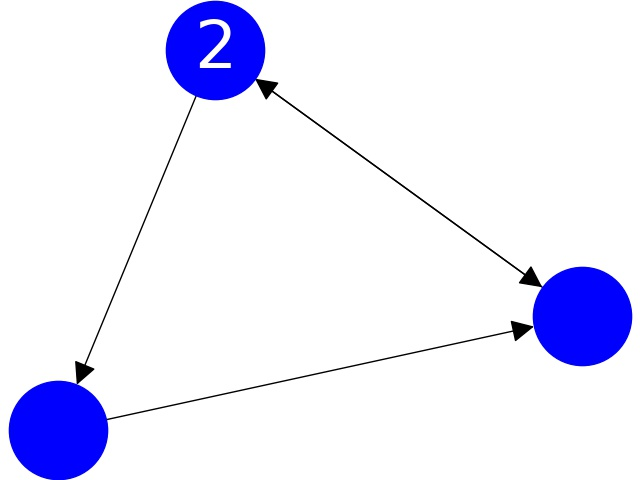
\includegraphics[width=\linewidth]{sandpile_simple_4}
    \caption{$c_{4} = (0,0,2)$}
  \end{subfigure}
  \begin{subfigure}[b]{0.3\linewidth}
    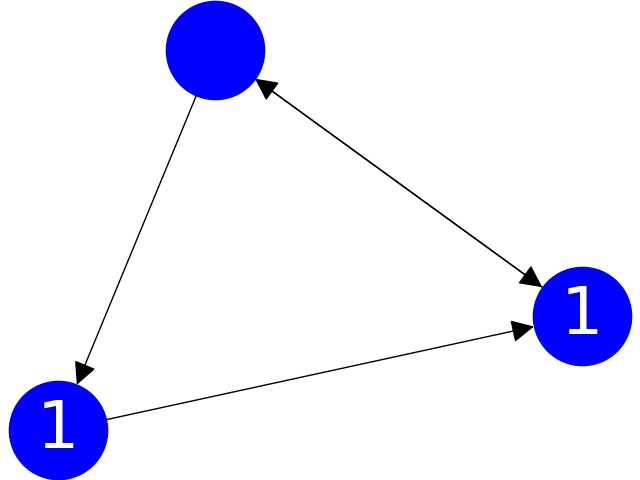
\includegraphics[width=\linewidth]{sandpile_simple_1}
    \caption{$c_5 = c_{1} = (1,1,0)$}
  \end{subfigure}

\end{figure}

\end{frame}




\begin{frame}
\frametitle{A Sink Vertex}
  \begin{itemize}
    \item A vertex $v$ of $G$ with no outbound edges ($e_v = {}$) is known as a \textbf{sink}.
    \item ``Sink'' vertices \textbf{never} fire.
    \item If every vertex has a direct path to a sink it is the \textbf{universal} sink.
    \item Every configuration on a directed graph with a universal sink stabilizes.
    \item From now on, all graphs will have a universal sink.
  \end{itemize}
\end{frame}


\begin{frame}
\frametitle{Sink Example}


  \begin{figure}[h!]
    \centering
      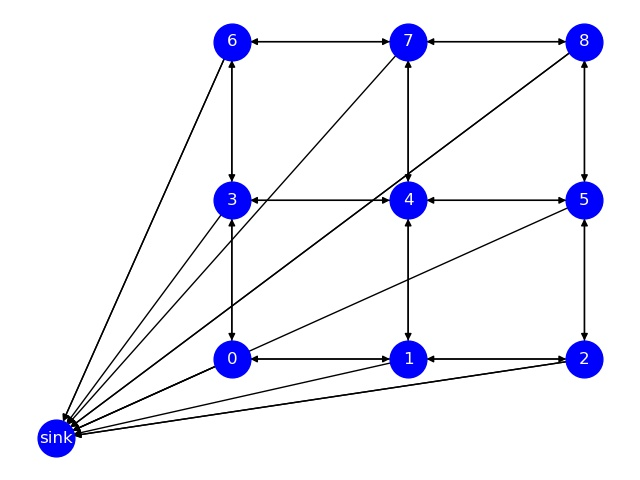
\includegraphics[scale=0.45]{sandpile_base}
      \caption{Directed graph with a sink.  $|e_{v_i}| = 4$ for all non-sink vertices.
      Vertices are labeled with their index/ID.}
  \end{figure}
\end{frame}

\begin{frame}
\frametitle{Chip Configuration Revisited}
  \begin{itemize}
    \item The sink vertex is excluded from the configuration vector
  \end{itemize}

  \begin{figure}[h!]
    \centering
      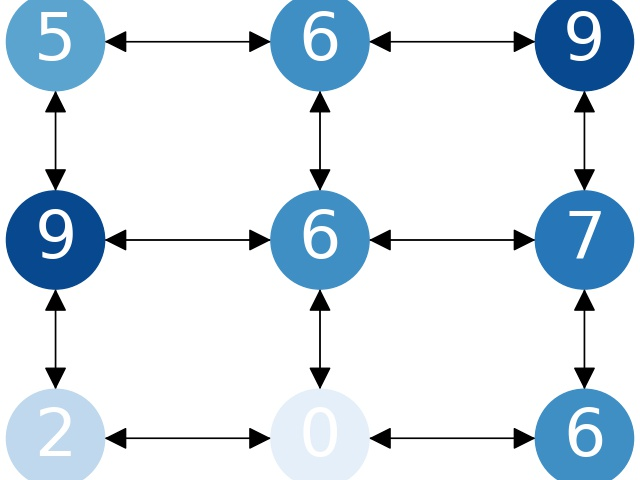
\includegraphics[scale=0.25]{sandpile_rand_state_0}
      \caption{$c_t = (2,0,6,9,6,7,5,6,9)$, indexed as on previous slide.}
  \end{figure}
\end{frame}


\begin{frame}
\frametitle{Reduced Laplacian}
\begin{itemize}
  \item $D$ is the out-degree matrix of $G$:
  \[
  D_{i,j} = \left \{
  \begin{tabular}{rl}
    $|e_{v_i}|$ & : $i = j$ \\
    $0$ & : $i \neq j$
    \end{tabular}
    \right.
  \]

  \item $e_{v_i,v_j}$ = edges from ${v_i}$ to ${v_j}$
  \item $A$ is the adjacency matrix of $G$:
  \[
  A_{i,j} = \left \{
  \begin{tabular}{rl}
    $|e_{v_i,v_j}|$ & : $i \neq j$ \\
    $0$ & : otherwise
    \end{tabular}
    \right.
  \]


  \item The \textbf{reduced Laplacian} is the matrix $L = D - A$ with rows/columns
  corresponding to the sink removed.

\end{itemize}


\end{frame}



\begin{frame}
\frametitle{Reduced Laplacian Example}

\begin{tabular}{cc}
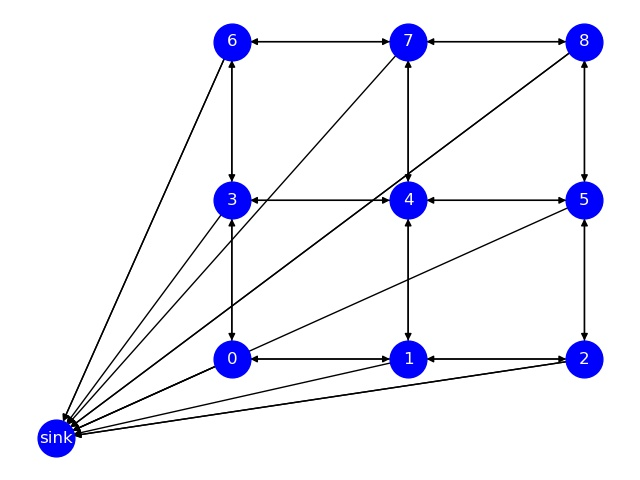
\includegraphics[scale=0.15]{sandpile_base}
&

 \\
 &   $L = \left(
  \begin{tabular}{ccccccccc}
  4&-1&0&-1&0&0&0&0&0\\
  -1&4&-1&0&-1&0&0&0&0\\
  0&-1&4&0&0&-1&0&0&0\\
  -1&0&0&4&-1&0&-1&0&0\\
  0&-1&0&-1&4&-1&0&-1&0\\
  0&0&-1&0&-1&4&0&0&-1\\
  0&0&0&-1&0&0&4&-1&0\\
  0&0&0&0&-1&0&-1&4&-1\\
  0&0&0&0&0&-1&0&-1&4
  \end{tabular}
  \right)$

\end{tabular}
\end{frame}


\begin{frame}
\frametitle{Firing and the Reduced Laplacian}

\begin{itemize}
\item Let $L_i$ be the row of the reduced Laplacian corresponding to $v_i$
\item If vertex $v_j$ fires at time/iteration $t$:
\[ c_{t+1} = c_t - v_j \]
\item $L_4 = (0,-1,0,-1,4,-1,0,-1,0)$
\end{itemize}

\begin{tabular}{cc}

  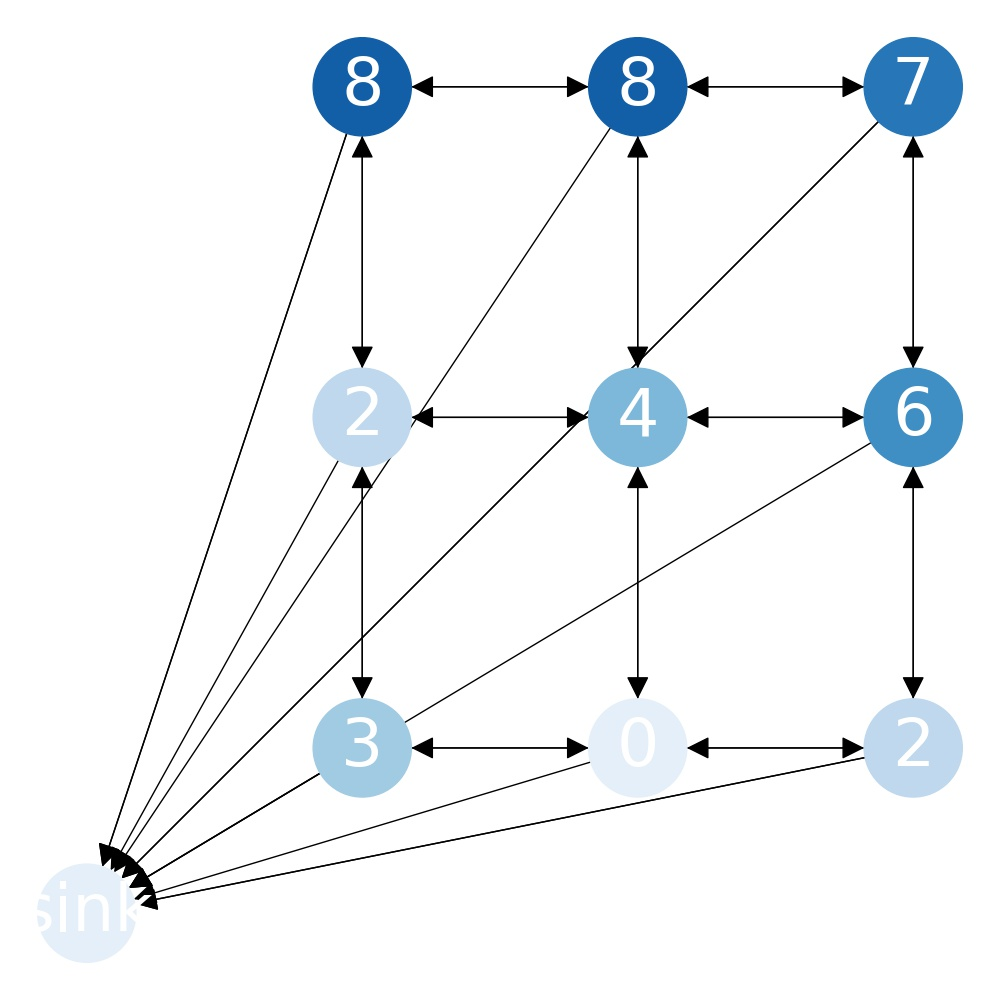
\includegraphics[scale=0.15]{sandpile_12}

  &   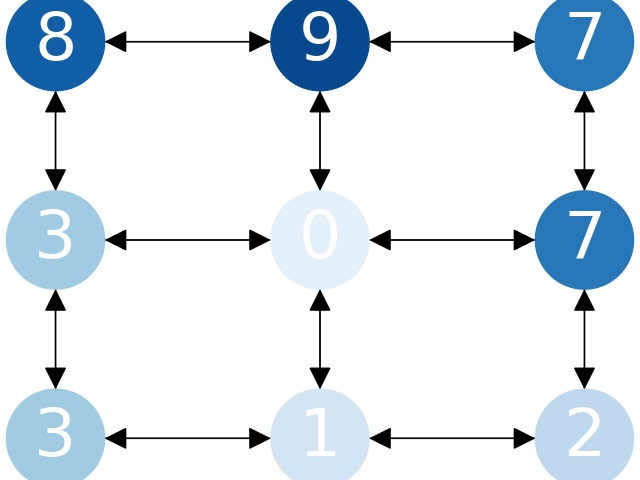
\includegraphics[scale=0.15]{sandpile_13}\\



$c_t = (3,0,2,2,4,6,8,8,7)$  & $c_{t+1} = (3,1,2,3,0,7,8,9,7)$

\end{tabular}



\end{frame}



\begin{frame}
\frametitle{Stabilizing Flipbook}

\end{frame}


\end{document}

[0, 1, 2, 1, 0, 2, 3, 3, 4, 4, 1, 5, 4, 5, 6, 3, 0, 6, 7, 7, 4, 5, 2, 1, 7, 6, 3, 4, 8, 8, 5, 7, 8]
{0: 3, 1: 4, 2: 3, 3: 4, 4: 5, 5: 4, 6: 3, 7: 4, 8: 3}


\begin{frame}
\frametitle{Firing ``History''}
\begin{itemize}
\item
\end{itemize}
\end{frame}

\begin{frame}
\frametitle{Chip Addition Operator}
\begin{itemize}
\item
\end{itemize}
\end{frame}







\begin{frame}
\frametitle{}

\begin{itemize}
\item
\end{itemize}

\end{frame}
